% Rust
\chapter{Rust - a new system level programming language}

To better understand where Rust, a new system level programming language, is placed among others of its kind, it is necessary to understand the difficulties that can arise by using them. Described by Bjarne Stroustrup, the creator of C++, in his book \textit{'The C++ programming language'}, one purpose of a programming language is to provide "a vehicle for the programmer to specify actions to be executed by the machine". That is even more true for a language that is used to create software that needs to utilize the underlying hardware very well to run at a good performance level. C++, and now Rust, are languages that provide the tools a programmer needs to write code that runs well on the hardware. But because that tools grant great power and control, any error done when implementing an application can be costly and have severe consequences. And there are two problems that, based on history and experience, prove quite difficult to solve. That problems are writing \textit{secure} and/or \textit{multi-threaded} code.
Secure code is often related to memory management and with languages that allow for manually controlling memory operations, the complexity of this issue increases. Consequences of these difficulties are security vulnerabilities and exploits, that also affected bigger companies without mentioning any names.
Although multi-threaded code does not that often cause security holes, the complexity, introduced by its parallel and asynchronous fashion, is the reason for errors that are hard to identify or even reproduce.

Rust tries to solve exactly this issues while claiming to maintain performance similar to the one of C or C++. Rust is developed by Mozilla and an open source community. It allows the programmer to manage the memory used by the application manually and tries to uphold a close relationship between language operations and the machine's hardware. While trying to solve problems that can occur in code written in C++, Rust shares several common principles with it. One of them being the ambition Bjarne Stroustrup has expressed for C++ in his paper \textit{"Abstraction and the C++ Machine Model"}:

\begin{quote}
	In general, C++ implementations obey the zero-overhead principle: What you don’t use, you don’t pay for. And further: What you do use, you couldn’t hand code any better.
\end{quote}

While following this and other principles shared with C++, Rust adds own standards it wants to uphold, including memory safety or simplified and trustworthy concurrency. To meet these promises, Rust relies heavily on compile-time checks that collaborate well with its static type system. 
In statically typed languages, the types of variables are checked at compile-time by a part of the compiler called the type-checker. Because those checks are not performed at the program's runtime, these languages are said to be \textit{statically type checked}. This comes with the advantage of allowing certain runtime checks to be omitted, which removes execution overhead and reduces the binary size. To prevent a common misunderstand when talking about statically typed languages, it has to be mentioned that \textit{type inference} does not prevent static type checking. Type inference is a language feature, that allows the programmer to omit any specific type when declaring a variable. The type is chosen by the compiler based on the context within a variable was declared and by knowing the type of the value that was assigned to it. 

Combined with its novel ownership system, that allows the definition of lifetimes for used values, it ensures memory safety without the need of a garbage collector. A garbage collector is a system that tracks memory allocations at runtime and manages their lifetime instead of the programmer. It is commonly used in higher level languages such as Java or C\#, but the safety comes with a cost in performance. When ownership shall be transfered from one owner to the new one, Rust uses the concept of \textit{moving} and defines \textit{borrows}, that allow temporary usage of values without affecting their ownership. These techniques, which are later described in more details, build the basis for the memory safety in Rust. They also provide the foundation Rust's concurrency model is built upon. Again, by using compile-time checks, Rust is able to detect certain problems related to multi-threaded code before the program is run once. 

This section continues with a description of Rust's current state and its ecosystem, followed a detailed description of the concepts that defined the language. They are explained and illustrated with code examples to built a better understanding. The shown code samples are compared to corresponding ones in C++, to show the difference between those languages.

\section{Language's current state}

With version 1.0 being released in 2014, Rust is a rather young programming language. The current version is 1.25.0, which was shipped on March 29, 2018. Examining the release notes and corresponding dates, it can be observed that about every six weeks a new major version upgrade is released. Version upgrades include \acp{RFC} issued by the community or by dedicated working groups. Another source of feedback for the language comes from the developers of \textit{Servo}, a new web browser engine entirely developed in Rust, which is developed by Mozilla. Servo powers the newest version of the Firefox browser and serves as a real-world test of Rust. Beside the concepts already mentioned above, Rust is embedded into an ecosystem that includes many tools that simplify the live of a developer. The parts of the ecosystem are described in the following section.

\section{Rust ecosystem}

During the development process of Rust several tools, alongside the Rust compiler \textit{rustc}, were built to enhance Rust's development process. Together with libraries, or \textit{crates}, created and distributed by Rust developers all around the globe, they form the Rust ecosystem. Two of these tools, every Rust developer will use at least once, are called \textit{Rustup} and \textit{Cargo}. 

\subsection{Rustc - The Rust compiler}

The Rust compiler went through many iteration steps until it reached its current state. The first version of the Rust compiler was written in OCaml, a different programming language using a functional, imperative and object-oriented style [OCAML]. It was the purpose of that compiler to compile a state of Rust that is capable of build a good compiler on its own, paving the way to a self-hosted compiler. A compiler that is self-hosted is written in the same language it normally parses. After Rust has reached the quality needed to serve that purpose, the legacy OCaml compiler was deleted from the language repository, which is proved by traveling back in time in the Rust GitHub repository commit history. At \url{https://github.com/rust-lang/rust/commit/6997adf76342b7a6fe03c4bc370ce5fc5082a869} it can be seen that the OCaml compiler part was removed. Beside the fact that the Rust compiler is self-hosted another interesting fact is how the compilation process works and what tools are included withing it. While \textit{rustc} serves as the compiler front-end, \ac{LLVM} is used in the compilation process and as a back-end. \ac{LLVM} is an open source tool for building programming languages and compilers. It includes many different tools and is a fundamental part of the compilation process of Rust programs.

\subsubsection{Compiler design \& LLVM}

Because \ac{LLVM} is such a fundamental part of the Rust compiler, this section is going to shortly describe how a classical compiler is designed and how the \ac{LLVM} project works.
The most popular design of a static compiler separates itself into three major components: the front-end, the optimizer and the back-end. It is the front-end's job to parse the code written in the source language, building an \ac{AST} out of it and reporting errors encountered during the processing. The optimizer is executed after the front-end finishes and applies transformations based an rules to enhance the performance of the code fed to it. After being optimized the code is then passed to the back-end, which is responsible to emit instructions matching the target architecture. Due to that reason the back-end can be also called \textit{code generator} in other literature. An illustration of such a three-pass-compiler approach can be seen in Figure \ref{fig:compiler_design}.

\begin{figure}[h!]
	\centering 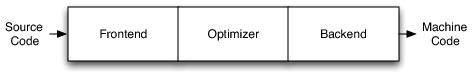
\includegraphics[width=\linewidth]{PICs/compiler_design.png}
	\caption{The stages of a three-pass compiler showing the way from source code to machine code}
	\label{fig:compiler_design}
\end{figure}

The biggest benefit from such an approach is that in theory it is simple to support different programming languages or machine architectures. If another language should be supported, this can be achieved by implementing a front-end for it while the optimizer and all existing back-ends just work without any big changes. The same applies for new target architectures, each requiring a new back-end, that supports every existing front-end out of the box. A good example for an open source compiler that supports several front-ends and back-ends is the GCC. But although the three-pass compiler design is well documented in various literature, in practice it is rather hard to uphold the separation all the time and several well-known open source projects did not do so. Due to that fact, \ac{LLVM} was created to unify and simplify the process of building languages and compilers. It shall also enhance the development of already existing languages. \cite{LLVM_ARCH}

One of the most important parts of \ac{LLVM} is its \ac{IR}. The \ac{LLVM} \ac{IR} is how code is represented in the compiler. The purpose of the \ac{IR} is to allow the compiler's optimizer to run mid-level transformations and analyses, while being a first class language with well-defined semantics on its own. The \ac{IR} in \ac{LLVM} serves as a perfect working environment for an optimizer, which is not constrained to any language or target specification. Beside the \ac{IR}, \ac{LLVM} uses a classical three-pass design. The front-end parsed the source code and generates \ac{LLVM} \ac{IR} from it, which is then handed to the optimizer for running several analysis and transformation passes. At the end all \ac{IR} code is passed to the back-end, where native machine code is generated from it. The implementation of \ac{LLVM}'s three-pass design can be seen in Figure \ref{fig:llvm_design}.

\begin{figure}[h!]
	\centering 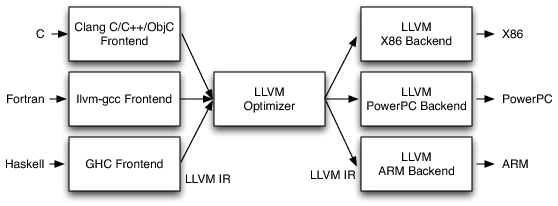
\includegraphics[width=\linewidth]{PICs/llvm_design.png}
	\caption{LLVM's implementation of the classical three-pass compiler design}
	\label{fig:llvm_design}
\end{figure}


\noindent
By using \ac{LLVM} during the compilation process, Rust gets all the benefits from already implemented optimizations in the \ac{LLVM} project. It is also responsible for the cross-platform abilities of \textit{rustc}, that is able to build binaries for different platforms specified by the compiler's toolchain.


\subsection{Rustup}

Rustup is a tool that helps installing the Rust toolchain. It allows the installation of different configurations and makes it possible to easily switch between several states of the Rust compiler. Beside being able to switch between nightly, beta and stable compiler versions, it is responsible for keeping them updated. It is currently able to run in all platforms, that are supported by Rust. With \textit{rustup} it is possible to install and manage several different Rust toolchains, managing them by a single set of tools. A toolchain in that context describes a single installation of \textit{rustc}.

Another important task of \textit{rustup} is the possibility to install additional targets for cross-compilation. Cross-compilation describes the process of generating compilation binaries for one machine (\textit{host platform}) on another, different one (\textit{build platform}). Because \textit{rustup} only installs the standard library binaries for the current platform, it is necessary to download them for the \textit{host platform} as well if the binaries shall be cross-compiled.

\subsection{Cargo}

Cargo is the package manager of the Rust programming language. Some of its features include downloading project dependencies, building the application, packaging crates and uploading them for distribution. It can be compared to package managers from other languages such as NPM from NodeJs or Nuget and C\# that are also capable of handling project dependencies in an automated fashion. But what makes Cargo rather unique and powerful are the capabilities it provides beside dependency management. It incorporates a build environment for Rust applications that is powerful and enhances the development process. Beside being able to invoke \textit{rustc} or a custom build script/tool, it is possible to test and benchmark a Rust application without any external tools. While other languages need to integrate that tools themselves , which often requires some amount of extra work, Cargo provides this important utilities out of the box.

Cargo is also the tool used to upload packages, or crates, to \textit{crates.io}, the Rust community;s package registry. Crates.io serves as a hub for many different libraries that can be used by any Rust application by simply depending onto them in the application's configuration file.

\section{Basic syntax}

Rust's syntax is quite similar to the one of C and even C++ in some parts. This section is going to showcase the its basic syntax based on examples to better understand the following concepts and code samples. It will also introduce some basics that are part of Rust's safety guarantees. 

\subsubsection{Variables, types \& mutability}

Because Rust is a statically typed programming language, every variable needs to have a distinct type specified at compile-time. As already mentioned the ability of type inference is not contradictory to statically typing. In Rust, the type of a variable can be annotated explicitly or inferred by the compiler. A variable declaration beginning with the \texttt{let} keyword do not require the programmer to specify the type, although it is not restricting an explicit declaration. Other variable declarations using \texttt{const} or \texttt{static} require a type to be annotated.\\

\begin{lstlisting}[caption={Variable bindings and mutability declarations in Rust}, label={lst:rust_var_bindings}, language=C]
	///
	/// Several variable bindings where both versions, type inference and type annotations, are showcased.
	/// The third binding will emit a warning because Rust sees that the literal exceeds the range of a 'u8'
	///
	let inferred  = 10;
	let annotated: u32 	= 42;
	let annotated_second: u8 = 1024;
	
	///
	/// Variable bindings with different mutability annotations
	///
	let immutable_var = 10;
	// immutable_var = 11 --> compilation error
	let mut mutable_var = 41;
	mutable_var = 42;
	
	///
	/// Rust does not allow implicit conversions between numerical types, 
	/// hence they have to be cast explicitly
	///
	let small_int: u32 = 100;
	let bigger_int: u64 = small_int as u64;
	
\end{lstlisting}

\noindent
As it can be seen in listing \ref{lst:rust_var_bindings}, Rust defaults all variable bindings to be immutable. Contradictory to C++, where immutable variables have to be marked as \texttt{const}, Rust requires the programmer to specify which variables are mutable by using the \texttt{mut} keyword.
Another situation where Rust prefers explicitness over implicitness is when casting between different types. Where in C++, numerical types can be implicitly converted to each other, Rust does not include such capabilities on purpose. If a type conversion shall be performed the programmer has to cast one type to the other by using either the \texttt{as} keyword, for a safe cast, or the \texttt{transmute} function, for an unsafe cast working quite similar to the \texttt{reinterpret\_cast} in C++.

\subsubsection{Pattern matching}

Another syntactical and functionally interesting feature of Rust are its pattern matching structures. Rust provides the \texttt{match} keyword, that works quite similar to a \texttt{switch} statement in C++, but is more powerful. 

\begin{lstlisting}[caption={Match statement in Rust, allowing for complex pattern matching in each arm}, label={lst:rust_match}, language=C]

	///
	/// 1) A match statement with range-based matches
	///
	let arr = [1, 2, 3, 4, 5, 6];
	
	match arr {
		[2, ..]  => { println!("Match if value at [0] is 2") },
		[1 .. 4] => { println!("Starting with 1 and ending with 4") },
		_ => { println!("Needed to handle every other case") }
	};
	
	///
	/// 2) A match statement with conditional patterns that returns from every arm
	///
	let x = 10;
	
	let res = match x {
		1 | 9 | 10 => { println!("Match if x is either 1 or 9"); true },
		_ => { println!("Match if x is 10"); true},
	};
	
	///
	/// 3) A match statement using destructuring
	///
	
	struct Data { 
		id: u32,
		amount: u64, 
	}
	
	let workload: Data = Data { id: 1, amount: 10 };
	
	match workload {
		Data { id: bind_one, amount: bind_two } => println!("Processing id: {} with amount: {}", bind_one, bind_two),
	}
	
\end{lstlisting}

\noindent
Listing \ref{lst:rust_match} shows several use cases of the match statement. The first match showcases the ability of complex patterns where the arms match only arrays that values are in a specific order. These complex patterns can be combined with conditional expressions, shown in the second match, making a pattern matching a powerful tool. In the third match, the expression of the first arm uses \textit{destructuring} in order to bind the fields of the structure to variables, that can be used in the body of that arm.

\section{Ownership system}

Regarding ownership Rust promises that the decision over a value's lifetime is up to the user and that the program, in spite of the given freedom, will never use a pointer to an already freed object (dangling pointer). While C++ allows for flexible lifetime decisions it cannot guarantee that the program does never hit a dangling pointer because it's the user's responsibility to ensure that no pointer to an already freed object is used.
Some highlevel languages such as Java or C\# solve the dangling pointer problem by introducing a garbage collector that controls when exactly objects are freed. This technique however also introduces an impact in performance.
To cope with this problem and to avoid garbage collection Rust came up with its own concept of ownership. In C++ and other languages it is said that an object 'owns' some other value that it points to and the owner therefore has control over the value's lifetime. In Rust this implicit ownership rule was turned to an explicit one and the language enforces that a value just has a single owner that controls its lifetime. As soon as the owner is freed, or dropped in Rust terminology, the owned value is dropped too. One example of Rust's ownership model is its \texttt{Box$<$T$>$} type that is a pointer to a value of type \textit{T} that is stored on the heap. When a \textit{Box} goes out of scope and is dropped, it frees the space it has allocated too, avoiding an otherwise introduce memory leak. \cite[Chapter 4. Ownership]{ProgrammingRust}
Whereas C++ also has constructs, called smart pointers, to express ownership, Rust's model comes without the overhead of storing additional meta data at runtime. Smart pointers have to store data for knowing when it is valid to drop the resource. Instead of this runtime overhead, Rust's system has to advantage of avoiding this overhead at all by moving the ownership checks to the compilation stage.

\subsection{Moves}

In C++, when a user assigns a variable to another or passes it to a function by-value, a copy of the value is created. Rust has chosen a different approach and instead of copying values, they are moved. When a move occurs,  the previous owner transfers ownership to the destination and gets uninitialized. The destination now controls the value's lifetime and becomes the new owner. Move semantics also exist in C++ and were introduced in the C++11 standard allowing the programmer to define move constructors and move assignment operators. \cite{CppMove} With the rule of using moves as the default behavior for assignment Rust can allow cheap assignments and keep the ownership clear as well. One trade-off the developer has to pay is that a copy now has to be requested explicitly. To do so in Rust one can implement either the \texttt{Copy} or \texttt{Clone} trait. What exactly a trait is and how they interact with other part of Rust is described in a later section. For now a trait can be though of as an extension, that can be implemented for other types, allowing them to be use by other code parts only knowing the trait's \ac{API}. The first one describes its implementor as trivially copyable by a plain \texttt{memcpy} where the second option requires the caller to invoke the \texttt{clone} method that returns a new object. \cite[Chapter 4. Ownership]{ProgrammingRust}

\subsection{Borrows}

Beside owning pointers, such as a \texttt{Box$<$T$>$}, Rust also defines non-owning pointer types that are called \textit{references}. The major difference to owning-pointers is that a reference has no effect on the lifetime or ownership of the value it is pointing to. In Rust terminology the act of referencing a value is called \textit{$'$borrowing$'$} and the compiler enforces that no reference outlives its referent. There are two kinds of references in Rust -- \textit{shared} and \textit{mutable} ones. A shared reference allows to read the value but not modify it and there can be as many shared references as the programmer needs. A mutable reference however is allowed to be read and modified but no other reference is allowed to be active at the same time. This concept introduces the compile-time rule of either several readers or one writer which is essential to the memory safety of Rust. One thing that shall not stay unmentioned is a big difference between C++ and Rust references. While under the hood both are just addresses, Rust references are allowed to be reseated after initialization whereas C++ references just alias the object they have been initialized with and cannot be reassigned afterwards. \cite[Chapter 5. References]{ProgrammingRust}

\subsection{Lifetimes}

With the knowledge on how Rust handles moves and references it is now possible to describe a more advanced feature of Rust's ownership model. To fulfill the promise of never using a dangling pointer in the entire program, Rust needs a way to tell, how long a value is valid or, in other words, alive. Although the Rust compiler is often able to deduce the lifetimes of objects or references from the context, there are some situations that require the programmer to opt-in. If such a situation occurs \textit{lifetime parameters} in the form of \texttt{'a}, where \texttt{a} is describing a distinct lifetime. Lifetimes enable the compiler to reason about how values are used and allow it to reject code, that would produce a dangling reference. One example where explicit annotation of lifetime parameters can be necessary is when returned references from functions. Such an example can be seen in the following code listing.\\

\begin{lstlisting}[caption={Returning a reference from a function, needing an explicit lifetime annotation. Compilation error because of a possible dangling reference.}, label={lst:fn_ref_lifetime}, language=C++]
fn get_element_from_slice<'a>(slice: &'a [u32], index: usize) -> &'a u32 {
	&slice[index]
}

/// ... Somewhere in the main function

let ref_to_element;
{
	let a_slice = [10, 20, 30, 42, 50];
	ref_to_element = get_element_from_slice(&a_slice);
}
assert_eq!(*ref_to_element, 42);

\end{lstlisting}

\noindent
As we can see, the function signature of \texttt{get\_element\_from\_slice} is providing a specific lifetime parameter \texttt{<'a>}, that is then connected to the parameter and return value, describing that they both share the same lifetime. With that constraint setup, it is said, that the reference returned by the function is not allowed to live any longer than the slice passed to the function. If the compiler now parses the part of the code that calls the function and then later uses the returned reference after \texttt{a\_slice} left the scope, the program would be rejected with an error and a hint that the slice the reference is pointing into is dropped while there was still a reference into it. The programmer is notified of this possible dangling reference at compile-time, which prevents application errors or undefined behavior at runtime. To solve the problem and make the code in Listing \ref{lst:fn_ref_lifetime} compile, only one line has to be changed. By moving the \texttt{assert\_eq!(*ref\_to\_element, 42)} two lines up into the scope, the reference returned does not live longer than the referee and the compiler will create a valid program.

Beside being needed for returned references explicit lifetime annotations are also necessary when creating custom types that hold references. Because the field of the type is still a reference, the Rust compiler needs to ensure its validity throughout the program the same way every non contained reference is checked. Due to that rule a struct that contains a reference to a value needs an explicit lifetime. The following listing displays how a simple example could look like.\\

\begin{lstlisting}[caption={Struct containing a reference to some value, needing a lifetime annotation to not create a dangling reference.}, label={lst:struct_ref_lifetime}, language=C++]
struct<'a> SomeData {
	pub reference: &'a u32,
}

/// ...

let instance;
{
	let x: u32 = 100;
	instance = SomeData { reference: &x };
}
assert_eq!(*instance.reference, 100);

\end{lstlisting}

\noindent
The code shown in Listing \ref{lst:struct_ref_lifetime} does not compile. The interested reader may already guess that the compilation error is related to a lifetime issue, which is in fact the reason. Because \texttt{SomeData}'s field \texttt{reference} needs a lifetime parameter and the instance was initialized with a reference to x, the struct's lifetime \texttt{'a} is bound to the one of \texttt{x}. It is then following the rules of every other reference and is not allowed to outlive its referent. Again to solve the issue with the code above, the usage of the reference has to be moved into the scope and therefore into the lifetime of \texttt{x}.

\section{Fearless concurrency}

The ownership concepts described in the previous section are very important for every Rust program. Because concurrent code tends to get complex quite fast if the number of threads rises, Rust's ownership concepts help reducing the complexity. Another advantage is the avoidance of concurrent bugs, which are hard to reproduce and debug. Because Rust wants to make concurrent programming more accessible by programmers it provides several features that are built upon design choices already used in concurrent programs. They allow a programmer to chose what style of parallelism is best for the current task and does not enforce the usage of a specific implementation. The following section will describe how one can create threads in Rust and what possibilities for communication and shared state there are.

\subsection{Threads \& immutable shared memory}

As almost every other system level programming language Rust offers an \ac{API} to create and manage threads. It is integrated into the standard library by the \texttt{thread} module. When a programmer needs to create a new thread this can be done by calling the \texttt{spawn} method and providing the function or closure, an anonymous function, it shall execute. The invocation of that function create an operating system thread, having its own thread local stack to store values. The handle returned by that function is later needed to \texttt{join} the thread. Joining is a common term for waiting until execution has terminated. That is needed to ensure that every thread is finished before the main thread terminates, which is ending the program.

Because a thread often also needs data it will operate on, there needs to be a way to provide both, mutable and immutable data. While writing to memory locations in a concurrent fashion needs some extra work for synchronization, read only access is simpler to control. Rust offers several abstractions to model a situation of shared ownership by providing reference counted types such as \texttt{Rc} or \texttt{Arc}. These special types are necessary due to the ownership concepts already introduced where a value can only have one owner at a time. But because moving and simple references do not work or cannot be checked for validity, reference counting is the way Rust implemented for shared ownership. So if a resource has to be shared among threads, it often is wrapped into an \texttt{Arc}, standing for atomic reference counted. Whenever another thread needs an instance of the wrapped data, the whole \texttt{Arc} is cloned, bumping its reference count by one. If all threads terminated and the reference count drops below one, it is dropped. These behavior is similar to smart pointer types, such as \texttt{shared\_ptr} or \texttt{unique\_ptr}, used in C++. This also prevents common concurrency bugs because the data inside an \texttt{Arc} is immutable. How resources are shared in a mutable way is described in the following section.

\subsection{Mutable shared state}

Multiple concurrent threads working on a mutable resource is a situation, that requires fine-grained access control to avoid critical bugs. Rust provides a system programmer with familiar concepts naming mutexes, conditional variables and atomics. These, so called \textit{synchronization primitives}, allow the programmer to synchronize the access of a mutable resource. In order to show some differences between the Rust approach and the one of other languages the \textit{mutex} primitive is described in more detail.

\subsubsection{Mutex}

A mutex is a synchronization primitive that guards resource or section of code from being accessed by more than one thread. The section that is protected by a mutex, or a lock in general, is referred to as a \textit{critical section}. Beside being used for thread synchronization, mutexes can be used for \ac{IPC} by using their named variants. A named mutex is visible across all processes of the \ac{OS} allowing them to communicate by changing its state. Using such a primitive in a language is nothing new and C++ also has an implementation in its standard library. A basic example of a C++ mutex can be seen in Listing \ref{lst:cpp_mutex} below. The code sample is simplified on purpose to show the usage of a mutex, though the global variables and meaningless mutation function.\\

\begin{lstlisting}[caption={Usage of a std::mutex to guard a critical section in C++}, label={lst:cpp_mutex}, language=C++]
std::mutex g_resource_mutex;
std::vector<int> g_shared_resource;

void mutate_shared_state() 
{
	g_resource_mutex.lock(); // Enter the critical section
	g_shared_resource.push(42);
	g_resource_mutex.unlock(); // Leave the critical section
}

int main()
{
	std::thread thread_1(mutate_shared_state);
	std::thread thread_2(mutate_shared_state);
	
	thread_1.join();
	thread_2.join();
}
\end{lstlisting}

\noindent
As the code sample above shows the mutex has to be locked and unlocked explicitly by the programmer whenever a shared resource is mutated. That section is only allowed to be run by a single thread at a time and every other one that tries to acquire the lock will be suspended and wait until the mutex is unlocked. Because a mutex is often strictly associated with an object or a resource, Rust came up with a slightly different \ac{API} for it, again turning an already commonly used implicit pattern into an explicit one. In Rust, the mutex wraps the data it protects and it can only be retrieved through the acquired lock. Therefore there is know way that the lock acquisition can be forgotten when the mutable resource is accessed. Listing \ref{lst:rust_mutex} shows how a mutex is created in Rust and how the data is retrieved by locking it.\\

\begin{lstlisting}[caption={Usage of a std::sync::Mutex to guard a shared resource in Rust}, label={lst:rust_mutex}, language=C++]
let guarded_vec: Mutex<Vec<i32>> = Mutex::new(vec![]);

// Somewhere in the concurrent function, accessing guarded_vec
let mut lock_guard = guarded_vec.lock().unwrap();
lock_guard.push(42);
\end{lstlisting}

\noindent
Contrary the \texttt{Mutex} in Rust is tightly bound to the resource it protects by wrapping it. Whenever \texttt{lock()} is called in the mutex,it returns a \texttt{MutexGuard} that is just a simple abstraction over a mutable reference to the wrapped type. Due to explicit implemented coercion traits on the mutex, it is possible to directly call methods of the wrapped type on the guard itself. A lock is then automatically released whenever the guard goes out of scope or if it is dropped manually, after access to the resource is not needed anymore.

\section{Polymorphism}

Polymorphism is a concept that is part of many programming languages for many years. In Rust it is implemented by \textit{traits} and \textit{generics}. While traits are a concept similar to interfaces or abstract base classes in C\# or C++ and allow for run-time polymorphism, generics are similar to C++'s templates, hence allowing for polymorphic behavior at compile-time. The following two sections are going to show how traits and generics work and how they are used in Rust.

\subsection{Traits}

A trait can be described as a set of functionality or features that a type, that is implementing it, supports. Traits are a powerful object to describe the capabilities of a type and combined with generics they can also be used to restrict the types that can be used with generic functions.\\

\begin{lstlisting}[caption={Example usage of a trait and a type implementing it}, label={lst:rust_trait}, language=C++]

trait ReadBuffer {
	fn read(&self, len: usize) -> Vec<u8>;
	fn valid(&self) -> bool; 
}

struct FileBuffer {
	buffer: [0; 100],
}

impl ReadBuffer for FileBuffer {
	fn read(&self, len: usize) -> Vec<u8> {
		// details omitted ...
	}
	
	fn valid(&self) -> bool {
		// details omitted ...
	}
}
\end{lstlisting}

\noindent
Listing \ref{lst:rust_trait} shows the trait \texttt{ReadBuffer} that exposes an interface to read values and to query for validity. The trait is then implemented for the distinct type \texttt{FileBuffer}, which implements the trait's methods to fulfill the purpose they describe. Now every instance of a \texttt{FileBuffer} provides the interface of the implemented trait. If another type would also implement the trait for itself, a function could take references to types implementing it while not needing to care what type exactly was passed to it. The code sample below shows a function that can work with any type that implements the specified trait. If a reference to any type implementing a trait is used it is called a \textit{trait object}.\\

\begin{lstlisting}[caption={A function, taking a trait object}, label={lst:rust_trait_object}, language=C++]
using ReadBuffer;

// 1) Calling read() on a trait object, every type that implements ReadBuffer (dynamic dispatch)
fn read_bytes(read_buffer: &ReadBuffer, length: usize) {
	let content = read_buffer.read(length);
}

// 2) Callind read() on a distinct type implementing ReadBuffer (static dispatch)
let file_buffer: FileBuffer = FileBuffer::new(file);
let content = file_buffer.read(100);
\end{lstlisting}

\noindent
Listing \ref{lst:rust_trait_object} shows two ways to invoke the trait's method on a type implementing it. In section one a function is taking a \texttt{\&ReaderBuffer}, called a \textit{trait object}, as argument. Trait object is the common term for a reference to a trait type. Because when using this approach the type behind the reference cannot be known at compile-time, Rust needs to store some additional information in order to call the right function. Behind the scenes, when using a trait object, a \textit{dynamic dispatch} is performed. To do a trait object is represented as a \textit{fat pointer}, containing the data and a so called \textit{virtual table pointer}, in memory. The virtual table pointer, or \textit{vptr} for short, contains information about the type behind the object. The concept is rather similar the one of C++ beside the fact that the \textit{vptr} is not part of the struct itself. This allows even types, that would otherwise be too small to hold an additional pointer, to implement traits.\\

\begin{figure}[h!]
	\centering 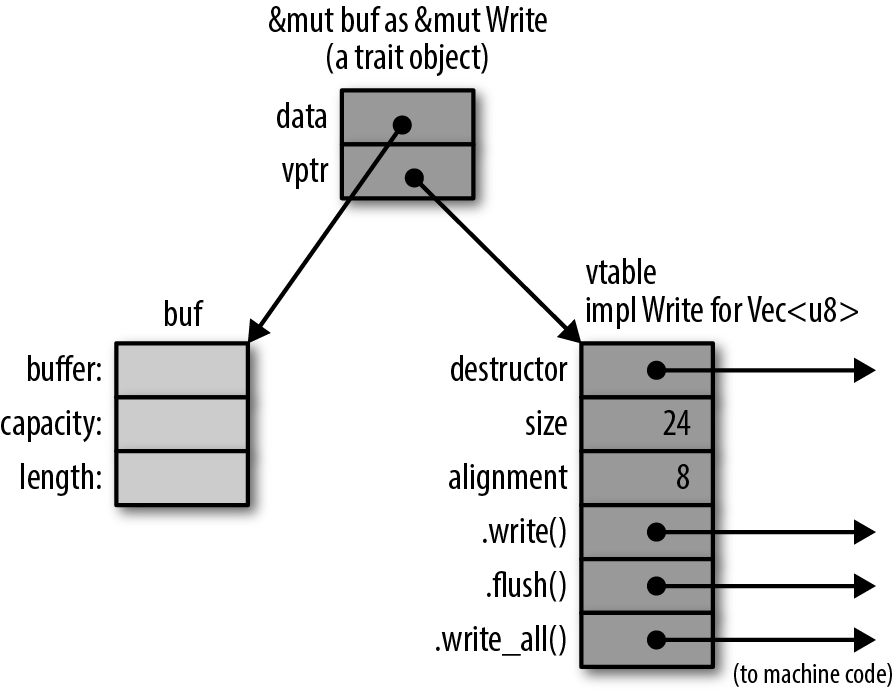
\includegraphics[width=\linewidth]{PICs/rust_vtable.png}
	\caption{Internal layout of a trait object in Rust. Dark grey parts are part of the vtable and only created once at compile-time}
	\label{fig:rust_vtable}
\end{figure}

\noindent
The above figure visually shows the described layout of a trait object. The image uses a trait called \texttt{Write} instead of the previously used \texttt{ReadBuffer}. The dark gray parts mark the parts that are hidden form the programmer. The vtable is created once for each type at compile-time and whenever a trait method is called via a trait object a lookup into the vtable is performed to find the location of the distinct type's implementation. As the interested reader now might already has guessed, calling methods through trait objects introduce an overhead.
That overhead can be avoided whenever the type of the trait's implementor is known upfront. If that is the case, as it is in Listing \ref{lst:rust_trait_object} in the second part of the code, the trait method can be called directly which is as fast as calling any other method.

\subsection{Generics}

Whereas traits and trait objects allow for runtime polymorphism, generics, similar to C++ templates, do the same at compile-time. By using \textit{type parameters} functions and structs can be turned into generic versions, usable with different types. One of the most popular examples of generic code is \texttt{Vec<T>} that works with many different types. The \texttt{T} in the type definition can be replaced by others, such as \texttt{Vec<u8>} or \texttt{Vec<String>}, allowing the vector to be adapted to the programmer's needs. Whenever the compiler discovers a type parameter for the vector it has now previously seen, it copies all of the vector's code with the T being replaced by the distinct type. This process is called \textit{Monomorphization} and also applies to generic functions.\\

\begin{lstlisting}[caption={A generic function in Rust showcasing trait bounds}, label={lst:rust_generic_code}, language=C++]
using ReadBuffer;
using std::fmt::Debug;

// Generic function with simple trait bound
fn read_from_buffer<T: ReadBuffer>(buffer: &mut T, len: usize) {
	let content = buffer.read(len);
	// ...
}

// Generic function, more complex trait bound
fn read_from_buffer_debug<T: ReadBuffer + Debug>(buffer: &mut T, len: usize) {
	let content = buffer.read(len);
	// ...
}
\end{lstlisting}

\noindent
Listing \ref{lst:rust_generic_code} above shows how generic functions can be declared. A feature not mentioned until now is the possibility of adding \textit{trait bounds} to a type parameter. A trait bound serves the purpose of requiring certain functionalities the types supplied to the generic function has to provide. Here can be a single trait or multiple once concatenated by a \texttt{+}. Whenever a type does not fulfill the bound it will raise a compiler error notifying the programmer about an unsatisfied trait boundary.

\section{Crates \& Modules}

The last feature of Rust that is going to be described in this chapter is the way Rust handles dependencies and structures code, both between different projects and in a single one. When coming from a C++ background the common way to structure a project is to generate different header files and include them wherever they are needed. While techniques such as include guards, checking that no file is included more than once per compilation unit, reduce errors made by programmers, adding several libraries to a project can get cumbersome quite fast. In the C++ world, when a library shall be added to the project, a programmer needs to add the include files first and then link against the necessary libraries. Contrary to this, Rust uses \textit{crates}, for sharing code between projects, and \textit{modules} for structuring code in one project. 

\subsubsection{Crates}

A crate is described as the collection of everything related to a single Rust project containing all source code, tests, examples, tools and so on. A Rust project can be dependent onto other crates that can be either come from \url{crates.io} or the same project. Then, when a Rust project is built with cargo, it fetches all dependencies first, compiling them with rustc into \textit{.rlib} files and then later statically linking them into the program. When using an external crate this is simply done by adding a \texttt{extern crate CRATE\_NAME} directive to the top of the project's main file and bring the necessary module into scope with the \texttt{use} keyword.

\subsubsection{Modules}

Where crates are used to share and manage dependencies between projects, withing a single one there are \textit{modules} to organize the code. A project can include multiple modules that can contain other ones or items, such as functions, types, variables and others. Modules can be compared to namespaces of other languages, serving as containers for logically grouped items. Modules are created with the \texttt{mod} keyword and can be nested into other ones. Additionally to the logical grouping, modules explicitly specify the visibility of contained items with either marking them as \texttt{pub} or not. Being marked as publicly visible allows the parts of the module to be used when the crate it contains is used, otherwise the non marked parts are just visible to the current module. Because modules can also be separated into several files, they are of great use when the size of a project grows and to design a meaningful \ac{API} for the user of the crate.

\section{Missing or unstable features}

Although Rust already provides many useful and important features a system programming language needs, the author recognized two features, that would have been rather important for the implementation part of the thesis, are currently not implemented or in an unstable stage. This section is going to shortly describe these missing features. It has to be mentioned that the selection is solely subjective in the author's opinion.

\subsection{Const generics} \label{rust_const_generics}

While coming from a C++ background the author missed a feature related to generic programming and that is often useful when working with templates in C++. Listing \ref{lst:cpp_const_generics} shows how that feature looks like in the world of C++, where it is called \textit{non-type template parameter}.\\

\begin{lstlisting}[caption={Showcasing template non-type parameters in C++}, label={lst:rust_generic_code}, language=C++]
template<typename T, size_t N>
class FixedSizeArray {
public:
	T* data();
	
private:
	T m_array[N];
}

int main() 
{
	FixedSizeArray<int, 100> hundredIntsArr;
	return 0;
}
\end{lstlisting}

\noindent
This above sample shows, how a template parameter, that is not a type, can be used to control the size of the array member. Non-type template parameters are a useful concept in generic programming when a variable parameter is known at compile-time. Unfortunately resembling such a behavior in Rust is currently not possible. There already is a \ac{RFC} and work is done in that field but at the moment there is no workaround to implement a similar approach. A description of that \ac{RFC} and a summary of related problems with the implementation can be found at GitHub under \url{https://github.com/rust-lang/rfcs/blob/master/text/2000-const-generics.md}.

\subsection{Placement-new functionality}

While the lack of const generics did not have a great impact onto the implementation of the submodules, the lack of a stable and working placement-new feature is rather bad. Placement construction describes a capability where it is possible for the compiler to construct aa value into a provided memory location. In C++, the \texttt{operator new} has a placement syntax, that allows the programmer to specify into which memory region the object shall be constructed.

\begin{lstlisting}[caption={Using placement-new to construct an object in a pre-allocated memory location}, label={lst:cpp_placement_new}, language=C++]
struct Data { ... };

char memory_buffer[sizeof(Data)];
Data* data = new (&memory_buffer) Data;
\end{lstlisting}

In Listing \ref{lst:cpp_placement_new} an instance of \texttt{Data} is constructed into a memory region on the stack by using the operator new with placement syntax. Its existence allows for efficient implementations of memory pools, garbage collectors and certain collection types.

At the beginning of the implementation period for this thesis, Rust had a nighlty feature for providing places where values could be constructed into. But during the first implementation of the memory system (\ref{mem_impl}) it was decided to stop development of it and remove all of its parts from the language. It is the author's opinion that the decision to remove the unstable version was a good one because beside of not being very ergonomic, the feature failed wo work in more cases than it was successful. Where it was capable of constructing a large array in-place it failed as soon as the array was the member of a struct. With this feature being removed from the language it was necessary to redesign the memory system and live with the drawbacks that introduced. One of the biggest disadvantages, that will be described in more detail in the next chapter, is the inability of allocating types that are too big for the stack and the overhead needed to move an object into the provided place instead of it being constructed there.

\section{Conclusion}

While being a rather young language, Rust already provides many features necessary for system programming. Combined with the design of \textit{rustc} and \ac{LLVM} as compiler back-end it is also useful for creating applications on multiple platforms. These two benefits are even more strengthened by the ecosystem and tool-suite that is build to supplement them. With Cargo and \url{crates.io} building applications and sharing them is a well-defined and documented process. With the basics of Rust and its ecosystem described, the next chapter will discuss the implementation details of the engine subsystems that were developed by the author during the process of this thesis.

